\section{The Transformation Framework}
\label{sec:trafo}

The core of the Visual Service Design Tool clearly is the transformation to executable code.  While by now the transformation to BPEL is the only one that can be conveniently used in practice, and thus will serve as an example later in this section, there are currently several other transformations under development.

The transformation framework has been designed from the very beginning to be as \emph{extensible} and \emph{reusable} as possible.  For that purpose the process of transformation has been subdivided into several stages, which are sequentially applied to the input model:
\begin{enumerate}
	\item \emph{Validation}: Validate the input model.
	\item \emph{Normalisation}: Prepare the input model for transformation.
	\item \emph{Structure Mapping}: Convert the input model to a block-like structure.
	\item \emph{Element Mapping}: Perform the actual mapping, create target model.
	\item \emph{Clean Up}: Remove redundancies, improve readability, etc.
\end{enumerate}

% Implementierungsdetails...
%The basic architecture can be seen in Figure~\ref{fig:trafo_framework}.  
The several stages are realised either as a set of graph transformation rules, a top-down pass through the input model, or a combination of both.  For the graph transformation rules the \emph{Tiger EMF Model Transformation} Framework~\cite{biermann2006graphica} (EMT) has been employed, providing a fast pattern matching and backtracking algorithm for EMF models.  In EMT, rules can be specified using a convenient graphical editor.  For the VSDT, however, the EMT has been modified so that instead of a Left Hand Side (LHS) with Negative Application Conditions (NACs) and a Right Hand Side (RHS), the rules feature an LHS, NACs and an \texttt{execute} method, which may contain arbitrary Java code.  Given the several cases to consider in BPMN this has proven more feasible.  The transformation is operating on a copy of the model to be transformed, which can be modified in the course of the transformation without affecting the original diagram.

%\begin{figure}%[htbp]
%	\centering
%	\includegraphics[width=\textwidth]{img/trafo_framework.png}
%	\caption{Essential classes of the transformation framework, including the BPEL case.}
%	\label{fig:trafo_framework}
%\end{figure}

\subsection{Stages of the Transformation}
\label{sec:trafo_stages}

%  Zielsprachen-Unabhaengigkeit von Validation, Normalisation und Structure Mapping
The Validation, Normalisation and Structure Mapping are to a great part independent of a specific target language, and in most cases the standard implementations provided with the transformation framework can be used.  However, it can be advantageous to extend them with additional checks and rules.

% Validation
For instance, in the \emph{Validation} stage, all identifiers are validated to contain only characters that are legal with respect to the given target language, which can be achieved by extending the standard implementation and using a respective regular expression for the validation of names.  Further, the validation includes a pass through the model, checking if each element needed is in place, thus reducing the number of checks necessary in the actual transformation, and providing clearer error messages to the user in case something is missing.

% Normalisation
The intent of the \emph{Normalisation} stage is to put the process diagram in a uniform form, and to transform it to what in the following will be referred to as the BPD's \emph{normal form}, a semantically equivalent representation of the diagram following more strict constraints than those given in the BPMN specification.  The transformation rules that are used in this stage are rather simple.  For instance, one rule will check if there are any Activities with multiple incoming or outgoing Sequence Flows attached to it, in which case a Gateway of type \textsc{xor} or \textsc{and}, depending on whether the Sequence Flows have any conditions, will be inserted in between.  Another rule will insert a ``no-op'' Activity in between any two Gateways that are directly connected by a Sequence Flow.  The advantage is that after the application of the normalisation stage there will be much fewer cases to consider in the structure mapping, which will be described in the next paragraph. A simple example of the consecutive execution of normalisation and structure mapping can be seen in Figure~\ref{fig:norm_struc}.

\begin{figure}%[htbp]
	\centering
	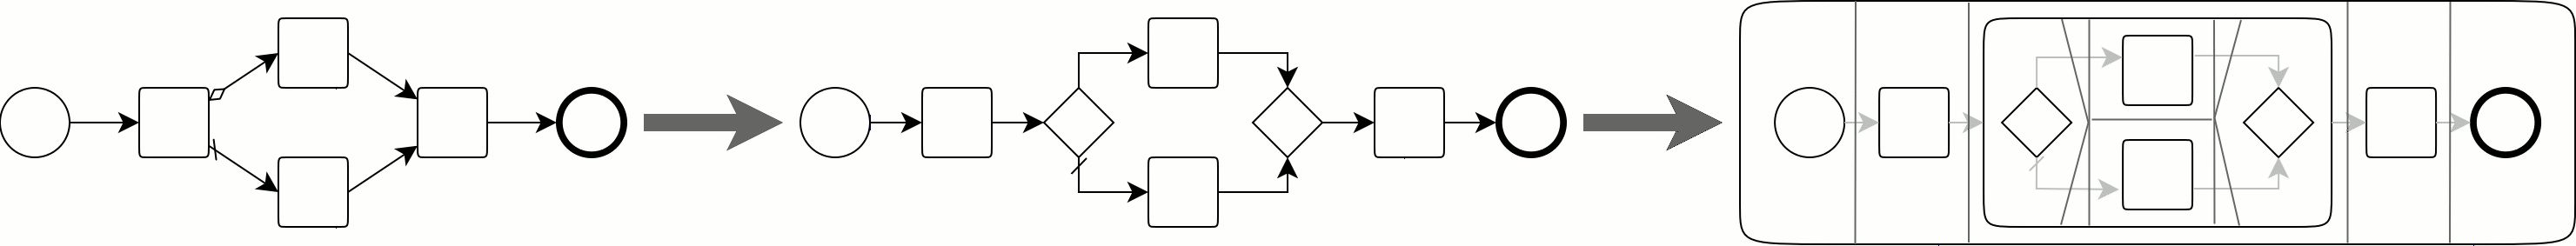
\includegraphics[width=\textwidth]{img/norm_struc_2.png}
	\caption{Simple example of normalisation and structure mapping.}
	\label{fig:norm_struc}
\end{figure}

% Structure Mapping
One of the challenges in transforming BPMN to executable languages is the mapping of the process model's graph-oriented structure to a more rigid block-oriented structure.  For that reason it is of great benefit making this part, the \emph{Structure Mapping}, independent of the actual target language, so it can be reused in mappings to other block-oriented languages.  We decided to follow a \emph{Structure Identification} strategy~\cite{mendling2005transformation}, being independent of BPEL's Link element.  As mentioned in Section~\ref{sec:editor_meta}, the transformation is using an extension of the BPMN metamodel used in the editor, allowing the introduction of additional elements representing sequences, blocks for parallel and alternative routing, loops, and event handler blocks, i.e.\ the basic building blocks of block-oriented languages.  Now, in the structure mapping stage, the model is searched for graph patterns which are semantically equivalent to these blocks, e.g.\ two Flow Object nodes connected with a Sequence Flow, or two Gateways connected by a number of branches of Flow Objects.  When such a pattern is found, it is replaced with the respective structured element, removing the involved Sequence Flow edges in the course, which are then no longer needed (their conditions, if any, are preserved in the newly created structured elements).  With these elements themselves being Flow Objects again, the rules of the structure mapping are applied until the entire process within each Pool has been reduced to a single complex element, e.g.\ a sequence, or until it can not be reduced any further due to structural flaws.  Some examples of BPMN graphs that can successfully be mapped to equivalent block structures and further to executable BPEL code can be seen in Figure~\ref{fig:structures}.  Of course, this stage can be adapted or entirely omitted, too, if the target language is structured differently.

\begin{figure}%[htbp]
	\centering
	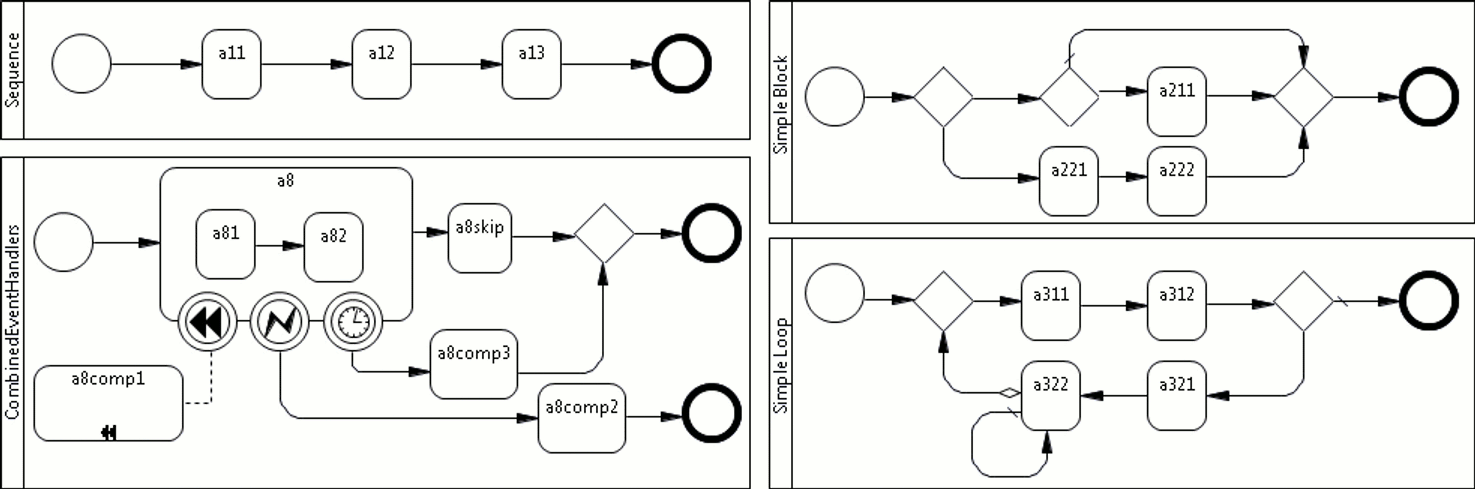
\includegraphics[width=\textwidth]{img/structures.png}
	\caption{Some examples of transformable BPMN graphs.}
	\label{fig:structures}
\end{figure}

% Element Mapping
After the rule-based structure mapping, in the \emph{Element Mapping} stage, the several BPMN elements can be mapped in a relatively simple top-down pass through the model.  We decided to use a top-down pass instead of rules in this stage, as it is faster and easier to maintain, but the framework does allow for other implementations as well.  As the element mapping is very dependent on the actual target language we will go further into detail later, regarding the transformation to BPEL.

% Clean Up
Finally, in the \emph{Clean Up} stage, a set of rules is applied on the newly created target model.  While this stage is optional, it can be of great use for improving the readability of the generated code while at the same time keeping the required logic out of the earlier stages.  For instance, nested sequences will be flattened, or sequences that hold a single element are replaced by that element itself.  Further, elements that resulted from no-op Activities inserted in the normalisation stage should be removed again in this stage.  As this stage operates on the target model, is has to be implemented anew for each target language.

For implementing a specific transformation, all that has to be done is to specify the element mapping, which can be done in any desired fashion by extending a special abstract class (see Figure~\ref{fig:trafo_framework}). In case the target language uses different block concepts, the structure mapping has to be adapted, too, but should still be reusable to some point.  In the majority of cases, implementing the other stages is optional.

\begin{figure}%[htbp]
	\centering
	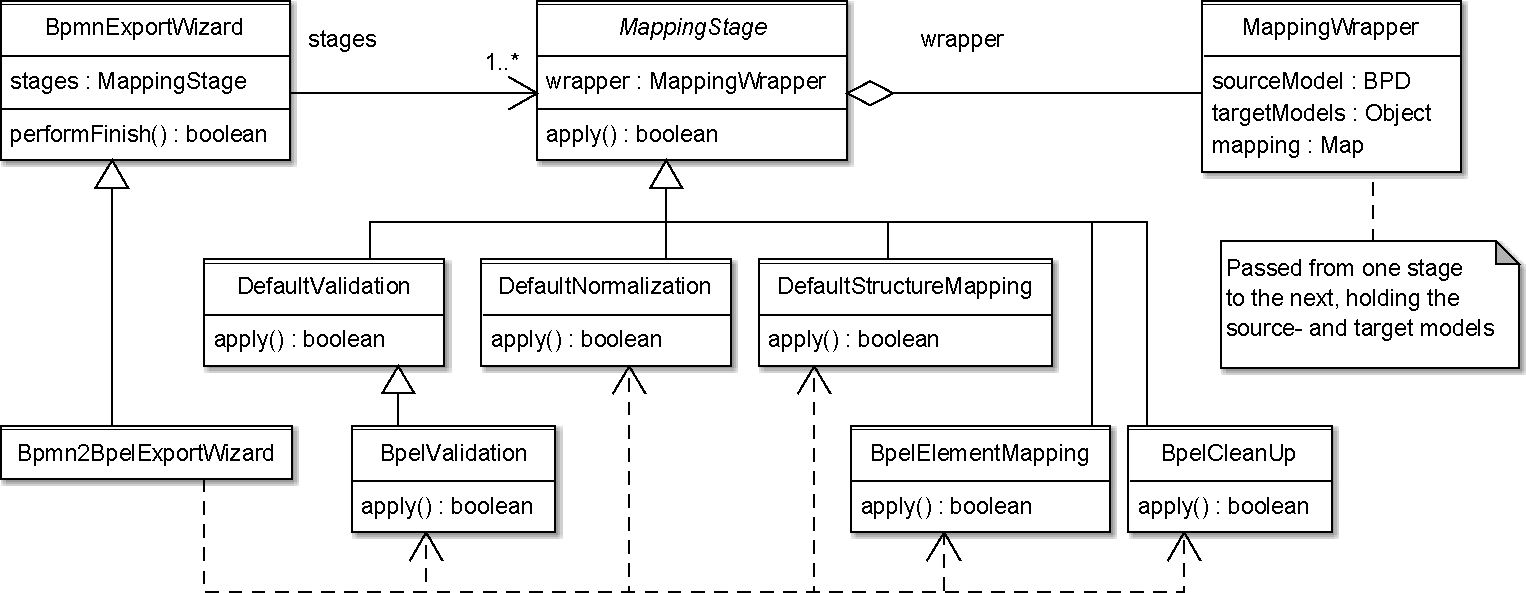
\includegraphics[width=\textwidth]{img/trafoframework.png}
	\caption{Essential classes of the transformation framework, including the BPEL case.}
	\label{fig:trafo_framework}
\end{figure}


\subsection{Transformation to BPEL}
\label{sec:trafo_bpel}

The transformation to BPEL presented in this work covers nearly the entire mapping as given in the BPMN specification~\cite[Chapter 11]{omg2006business}, including event handlers, inclusive \textsc{or} and event-based \textsc{xor} Gateways, just to name a few.  Still there are some elements for which the mapping is not given very clearly, such as \textsc{timer} Start Events, independent Sub Processes or multi-instance parallel loops.  While these elements will be transformed as described in the specification, the resulting BPEL processes will require some amount of manual refinement.  Besides the BPEL process files a WSDL definitions file is created, holding the message types derived from the process properties and the input and output messages and interfaces (port types) for the several Web services being orchestrated by the process.  Still, the WSDL's binding and service blocks and necessary schema types, if any, can not be generated automatically yet, due to insufficient information in the source model.  We are currently investigating ways of extending the BPMN metamodel in order to include more information in the model and at the same time making it more independent of the BPEL language.

In the validation used for the transformation to BPEL, all identifiers are tested to contain only characters that are legal with respect to BPEL.  Additionally all expressions used e.g.\ in Assignments and loop conditions are scanned for occurrences of Property identifiers.  So if a Process \texttt{Proc} has a Property \texttt{foo} and there is an Assignment with an expression like \texttt{"foo+1"}, the expression will be changed to \texttt{"bpws:getVariableData('Proc\_ProcessData','foo')+1"}.  Thus the user does not have to care about the way Properties are represented with messages in BPEL but can use a Property's plain name in expressions.


\subsection{Example}
\label{sec:trafo_example}

The following example will show one of the scenarios being used in a smart home environment in the SerCHo project.  The resulting BPEL processes were validated and tested with the \emph{ActiveBPEL} designer and process engine.\footnote{\url{http://www.activebpel.org}}

The BPMN diagram in Figure~\ref{fig:example} is showing a ``Light Alarm'' process, that is used to open the blinds in the user's room to wake her up in a more pleasant way than the usual alarm clocks do.  For that purpose, firstly information on the current weather is retrieved using an external Web service.  Thereafter, based on the weather data, either the sunblinds are opened, or the ceiling light is turned on, or both.  In case the user does not get up, which is checked using an RFID based localisation solution, the stereo is turned on, playing her favourite song or alternatively an unpleasant alarm sound.

\begin{figure}%[htbp]
	\centering
	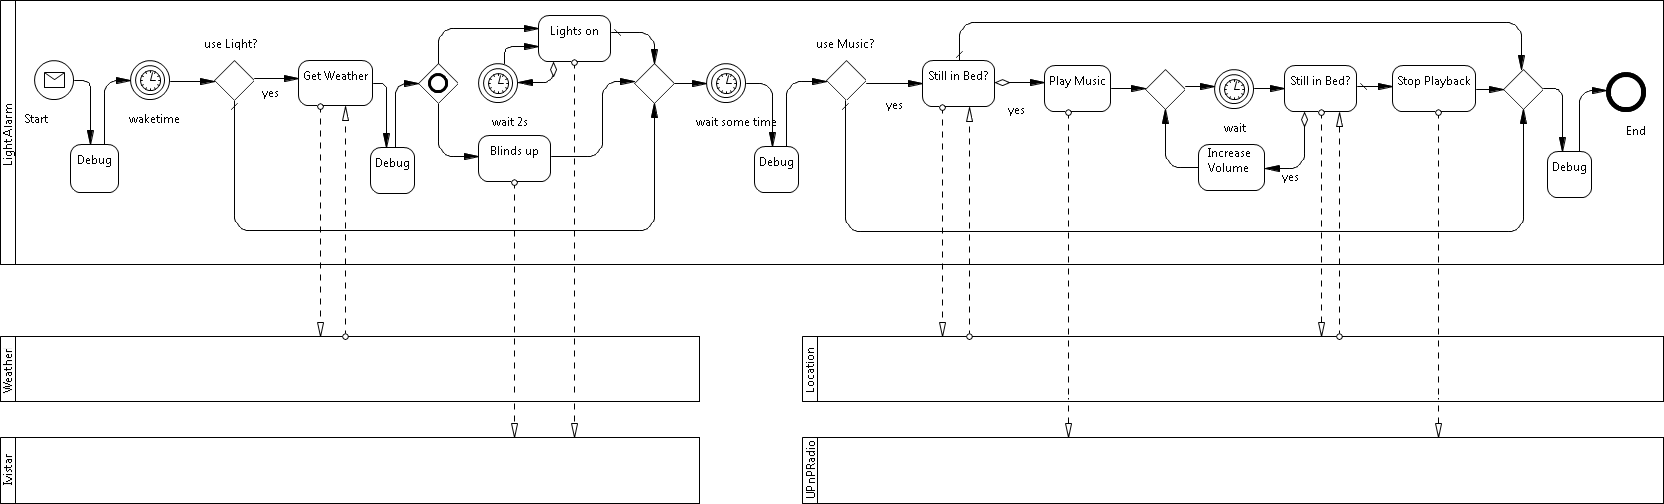
\includegraphics[width=\textwidth]{img/demo_lichtwecker_kompakt.png}
	\caption{``Light Alarm'' Example Process}
	\label{fig:example}
\end{figure}

For each of the above devices --- blinds, lights, localisation, and stereo --- Web service interfaces were written, so they can be integrated in a BPEL process.  While the WSDL file that is used by the process, holding the definitions for the various orchestrated services, has to be extended with the service bindings, the BPEL code resulting from this example is readily executable.


\subsection{Transformation to JIAC}
\label{sec:trafo_jiac}

Concerning our goal of transforming BPMN diagrams to multi-agent systems (MAS) the work is still at an early stage.  First, a \emph{normal form} for BPMN diagrams has been investigated, to facilitate the mapping~\cite{endert2007towards}.  Later, the first steps of the actual mapping have been developed, basically mapping Pools to agents, Processes and Flow Objects to the agents' plans and the control flow, and Message Flow to the exchange of messages between the agents~\cite{endert2007mapping}.

A first prototype targeting the agent framework JIAC IV~\cite{sesseler2002modularearchitektur} has already been implemented.  As the theoretical part of the mapping is not yet fully matured, there is still some work to do.  However, with the given transformation framework every addition to the mapping can quickly be adopted.

